\subsection{Model Transformations}

% MDD and MTs. Not very important but I do not know how far back should we start.
Model-Driven Development (MDD) is a software engineering approach that uses
models - typically represented as graphs - as first class citizens to create and evolve software systems
\cite{Hailpern:2006vd}.
Model Transformations, prescribed by Model Transformation Languages (MTLs) are the preferred approach to manipulate those models \cite{Software2003}.
MTLs typically describe a set of rules that guide the transformation of models.
Their productivity comes from the fact that those rules can be described elegantly without the accidental complexity of graph manipulation.

% Model translations vs Rewritting Transformations.
Here, a model transformation is defined as a translation, as opposed to a graph rewriting process.
In graph rewriting, a graph representing a model or a set of models gets rewritten continuously according to a set of rules, until some termination criteria is met. 
In a model translation, there is a source model and a target model and the target model is the result of applying the translation to the source model.
Operationally speaking, each of these approaches can mimic the other: graph rewriting can be used to perform model translations (e.g. \cite{Grunske2005}) and model translations, \emph{when applied repetitively}, can perform graph rewriting.

\subsection{The DSLTrans Transformation Language}

%DSLTrans: why it was used to prove properties.
DSLTrans~\cite{Barroca2011} is an MTL used to specify model translations.
Its main distinctive feature is that the model translations that are described in DSLTrans are guaranteed to always terminate\footnote{This result assumes that finite models are used.}. This feature comes at a cost: DSLTrans is not Turing complete, i.e., no unbounded recursion, non-determinist or element deletion
can be specified. Despite the apparent lack of expressivity, our experience has showed that it is possible to specify a wide range of transformations using DSLTrans. Furthermore, it makes DSLTrans transformations ideal to prove properties about since the set of possible behaviors is finite.

%Why use the families to persons example.
To present the syntax and semantics of DSLTrans, we will be using the Families-to-Persons transformation from the ATL transformation zoo \footnote{\url{http://www.eclipse.org/atl/atlTransformations}}.
Because this transformation can be easily understood, it allows us to focus on the essential concepts of DSLTrans.

%Metamodels of families to persons
Figure~\ref{fig:families_to_persons_metamodels} shows the metamodel of the Family language on the left, and the Community language on the right.
These two languages represent different perspectives of groups of people. A family has a father, mother, daughters and sons.
A community is composed of people and each person can either be a man or a woman.

\begin{figure}
        \centering
        \begin{subfigure}{0.5\linewidth}
                \centering
                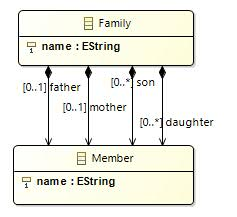
\includegraphics[width=\linewidth]{figures/Familiesclassdiagram}
                \caption{Families metamodel.}
                \label{fig:families_mm}
        \end{subfigure}%
        \begin{subfigure}{0.5\linewidth}
                \centering
                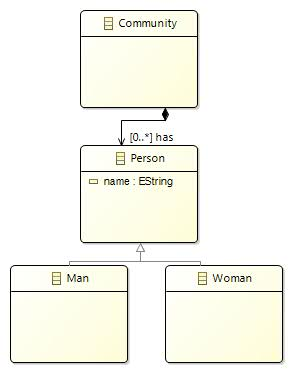
\includegraphics[width=\linewidth]{figures/communitydiagram}
                \caption{Community metamodel.}
                \label{fig:community_mm}
        \end{subfigure}%
        \caption{ }
        \label{fig:families_to_persons_metamodels}
\end{figure}

% Informal description of DSLTrans.
The partial translation of a family model into a community model, in DSLTrans,
is done by executing the transformation shown in Figure~\ref{fig:families_mm}.
We show the partial transformation because it is sufficient to explain DSLTrans
semantics. DSLTrans transformations are organized in partial ordered layers.
Each layer is executed after its previous layer. Each layer has a set of rules.
The execution of a layer means the execution of the rules that comprise that
layer.
The rules inside the same layer are executed independently of one another, i.e.,
there is no order of execution of rules and they cannot affect the execution
(e.g., enable or disable) of one another. Each rule has a match pattern and an apply pattern.
In Figure~\ref{fig:families_mm}, besides the input model description on the top,
there are two layers. The input model description contains the location of the
input model to be translated, which in this example is a family model. The first layer has two rules and the second layer
has one rule:
\begin{compactdesc}
	\item[FamilyRule] Find all the instances of Family and, for each one, create a Community element.
	\item[SonRule] Let $S = \left\{ (f, m_1) , \ldots , (f, m_n) \right\}$ be all instances, in the input model, of Family that are connected to instances of Member by the ``son'' association. This rule states that for each of those connected elements
$(f, m_i)$, create a Man element with a name defined by the concatenation of the name attribute of $m_i$ with the name attribute of $f$. Basically, it creates a man for each family member that is a son.
	\item[UnionManRule] Let $S = \left\{ (f, m_1) , \ldots , (f, m_n) \right\}$ be all instances of Family that are connected to instances of Member by the ``son'' association. 
	Now, let $R$ be the set formed by iterating each element $(f, m_i)$, finding the instance of Man ${man}_i$ that was created previously in SonRule and finding the instance $c$ of Community that was created in the FamilyRule. This rule iterates each element $(f, c, m_i, {man}_i)$ of the $R$ set and creates a ``has'' association between $c$ and ${man}_i$. The trace links are of paramount importance to connect the instances created in rules of the \emph{previous} layer.
\end{compactdesc}

\begin{figure}
\begin{center}
  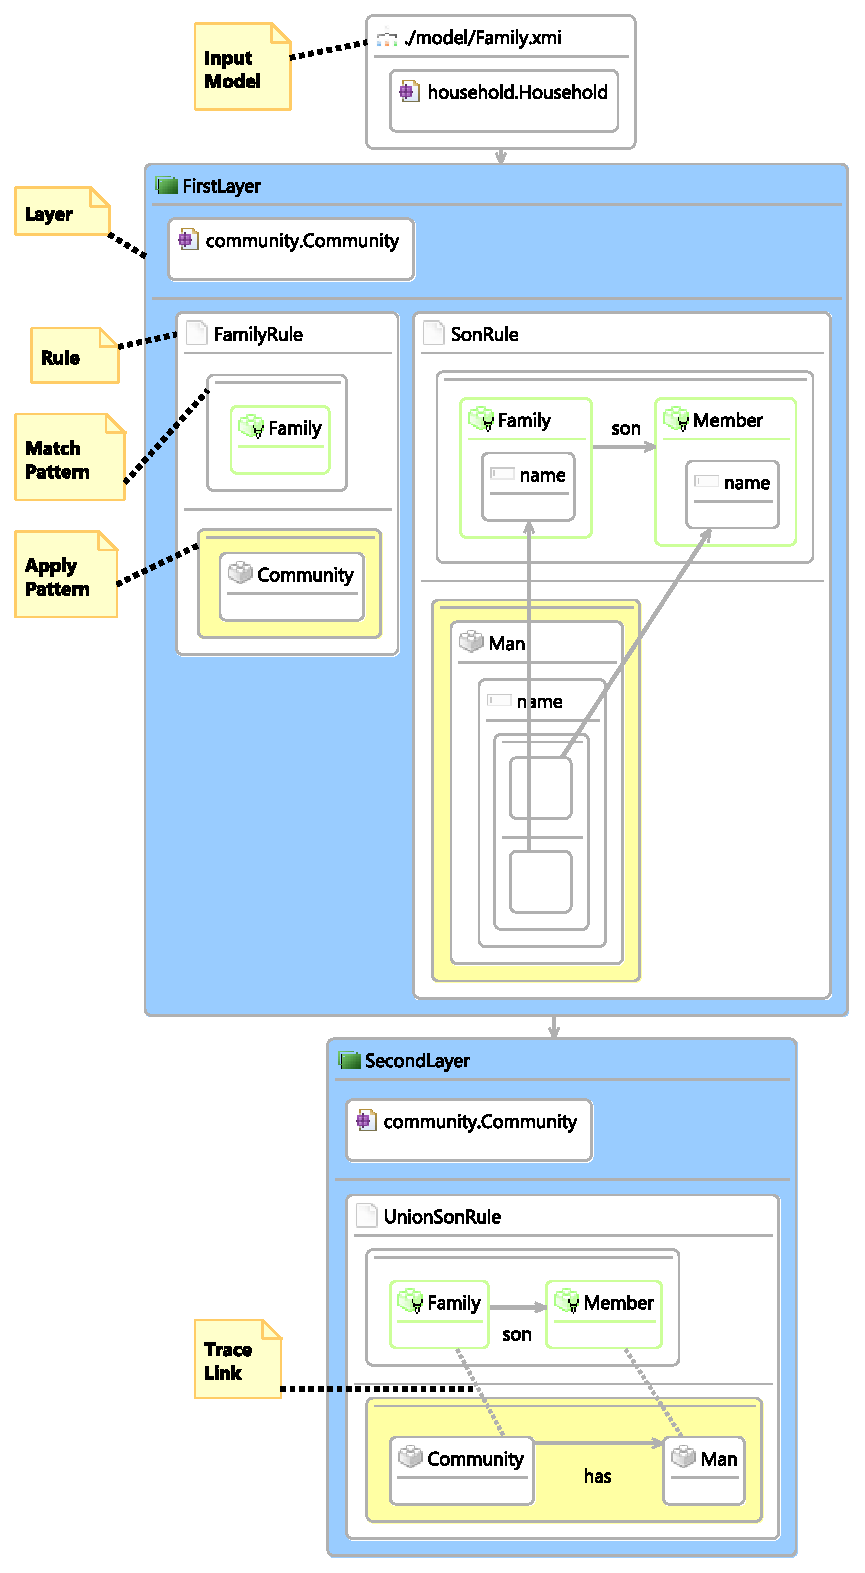
\includegraphics[width=0.35\textwidth]{figures/families_to_persons_hot2}
  \caption{DSLTrans transformation of Families to Communities (partial).}
  \label{fig:families_mm}
\end{center}
\end{figure}

%summary and bridge to the next section
In summary, if we apply the DSLTrans transformation partially shown in  Figure~\ref{fig:families_mm} to a family model with a father, a mother, a son and a daughter, we expect to get a community model with 2 men and 2 women. The previous sentence represents a property about the transformation that we might wish to verify automatically.

\subsection{Model Transformation Verification}

% What is transformation verification?
Notice that the previous property is in the form of an implication, which must be true independently of the concrete input model given to the transformation.
This means that to prove the property, it is not enough to prove that it holds for a single input model with a father, a mother, a son and a daughter. That would be just testing the transformation.
Rather, we must prove that it holds for the infinitely many possible input models.

% Motivation for automatic verification
For small transformations it is easy to prove that they satisfy certain
properties but model transformations have been successfully applied in industry
(e.g., \cite{daghsen:hal-00660252,Giese2010}) and these transformations - and
the models involved, as evidenced in \cite{Selim2012} and in our own case study
Section~\ref{sec:mbeddr_case_study} - can be quite large
\footnote{Transformations with circa 50 rules and metamodels with more than 1500
classes}.
For these transformations, automatically proving that they are correct is of utmost importance.

%bridge to the next section.
By correct transformations, we mean that they are automatically proven to satisfy the properties described by the domain expert. We abstain from prescribing which properties are of interest. Instead, we focus on the verification/proving process itself.



